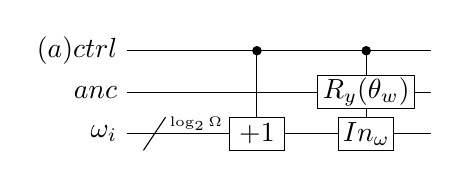
\begin{tikzpicture}[scale=1.000000,x=1pt,y=1pt]
\filldraw[color=white] (0.000000, -7.500000) rectangle (110.000000, 37.500000);
% Drawing wires
% Line 1: ctrl W \text{(a) }ctrl
\draw[color=black] (0.000000,30.000000) -- (110.000000,30.000000);
\draw[color=black] (0.000000,30.000000) node[left] {$\text{(a) }ctrl$};
% Line 2: anc W anc
\draw[color=black] (0.000000,15.000000) -- (110.000000,15.000000);
\draw[color=black] (0.000000,15.000000) node[left] {$anc$};
% Line 3: i W \omega_i
\draw[color=black] (0.000000,0.000000) -- (110.000000,0.000000);
\draw[color=black] (0.000000,0.000000) node[left] {$\omega_i$};
% Done with wires; drawing gates
% Line 5: i / ^{\log_2{\Omega}}
\draw (6.000000, -6.000000) -- (14.000000, 6.000000);
\draw (12.000000, 3.000000) node[right] {$\scriptstyle{^{\log_2{\Omega}}}$};
% Line 6: ctrl anc i LABEL width=-1
% Line 8: i G width=20 $+1$ ctrl
\draw (47.000000,30.000000) -- (47.000000,0.000000);
\begin{scope}
\draw[fill=white] (47.000000, -0.000000) +(-45.000000:14.142136pt and 8.485281pt) -- +(45.000000:14.142136pt and 8.485281pt) -- +(135.000000:14.142136pt and 8.485281pt) -- +(225.000000:14.142136pt and 8.485281pt) -- cycle;
\clip (47.000000, -0.000000) +(-45.000000:14.142136pt and 8.485281pt) -- +(45.000000:14.142136pt and 8.485281pt) -- +(135.000000:14.142136pt and 8.485281pt) -- +(225.000000:14.142136pt and 8.485281pt) -- cycle;
\draw (47.000000, -0.000000) node {$+1$};
\end{scope}
\filldraw (47.000000, 30.000000) circle(1.500000pt);
% Line 9: anc G:width=35 $R_y(\theta_w)$ i G:width=20 $In_\omega$ ctrl
\draw (86.500000,30.000000) -- (86.500000,0.000000);
\begin{scope}
\draw[fill=white] (86.500000, 15.000000) +(-45.000000:24.748737pt and 8.485281pt) -- +(45.000000:24.748737pt and 8.485281pt) -- +(135.000000:24.748737pt and 8.485281pt) -- +(225.000000:24.748737pt and 8.485281pt) -- cycle;
\clip (86.500000, 15.000000) +(-45.000000:24.748737pt and 8.485281pt) -- +(45.000000:24.748737pt and 8.485281pt) -- +(135.000000:24.748737pt and 8.485281pt) -- +(225.000000:24.748737pt and 8.485281pt) -- cycle;
\draw (86.500000, 15.000000) node {$R_y(\theta_w)$};
\end{scope}
\begin{scope}
\draw[fill=white] (86.500000, -0.000000) +(-45.000000:14.142136pt and 8.485281pt) -- +(45.000000:14.142136pt and 8.485281pt) -- +(135.000000:14.142136pt and 8.485281pt) -- +(225.000000:14.142136pt and 8.485281pt) -- cycle;
\clip (86.500000, -0.000000) +(-45.000000:14.142136pt and 8.485281pt) -- +(45.000000:14.142136pt and 8.485281pt) -- +(135.000000:14.142136pt and 8.485281pt) -- +(225.000000:14.142136pt and 8.485281pt) -- cycle;
\draw (86.500000, -0.000000) node {$In_\omega$};
\end{scope}
\filldraw (86.500000, 30.000000) circle(1.500000pt);
% Done with gates; drawing ending labels
% Done with ending labels; drawing cut lines and comments
% Done with comments
\end{tikzpicture}
